\documentclass[11pt,a4paper]{article}

% -----------------------------------------------------------------------------
% CS6868 Research Mini-Project Report Template
% -----------------------------------------------------------------------------
% Target length: 5-10 pages (including figures, excluding references).
% Compile with: latexmk -pdf main.tex
% -----------------------------------------------------------------------------

\usepackage[utf8]{inputenc}
\usepackage[T1]{fontenc}
\usepackage[margin=1in]{geometry}
\usepackage{microtype}
\usepackage{lmodern}
\usepackage{amsmath,amssymb}
\usepackage{graphicx}
\usepackage{booktabs}
\usepackage{array}
\usepackage{enumitem}
\usepackage{xcolor}
\usepackage{listings}
\usepackage{hyperref}
\usepackage[capitalise,noabbrev]{cleveref}

\hypersetup{
  colorlinks=true,
  linkcolor=black,
  citecolor=blue!60!black,
  urlcolor=blue!60!black,
}

% --- Listings style (for code snippets) ---------------------------------------
\definecolor{codegray}{gray}{0.95}
\lstset{
  basicstyle=\ttfamily\small,
  backgroundcolor=\color{codegray},
  frame=single,
  framesep=4pt,
  breaklines=true,
  columns=fullflexible,
  keepspaces=true,
  showstringspaces=false,
}
\setlength{\parskip}{0.5em}

% --- Title block --------------------------------------------------------------
\title{%
  \textbf{CS6868 Research Mini-Project} \\[0.3em]
  \Large An Investigation into Parallel Task Scheduling using Dynamic
  Circular Work-stealing Deques (An OCaml Implementation)
}
\author{%
  Alina Banerjee \\ \texttt{ns26z001@smail.iitm.ac.in}
  \and
  Ankita Das \\ \texttt{rollno2@smail.iitm.ac.in}
  \and
  Dhruvanshi \\ \texttt{rollno3@smail.iitm.ac.in}
}
\date{\today}

\begin{document}
\maketitle

\begin{abstract}

This project attempts to build a user-level task scheduler that can distribute
tasks to dynamic circular deques. Using this scheduler, we run a set of parallelizable
problems to measure
the efficiency of work-stealing across such deques. Work-stealing is a paradigm
where idle deques i.e. ones that have completed tasks allotted to them steal
tasks from other deques, thus rebalancing loads across deques and speeding up
overall program execution. At the same time, this introduces contention with
possibly multiple deques trying to steal from one that may be about to pick up
the same task for execution locally.

\cite{arora1998thread} originally introduced this idea of using array-based
deques (double-ended queues) for managing tasks across multiprocessors.
With fixed-size arrays, inefficient memory usage and array overflow were the
fundamental problems. Our
implementation is based on \cite{chase2005dynamic} which addressed both problems
using dynamic cyclic arrays: arrays that can grow or shrink in size as needed and
are cyclic which ensures the overflow problem is only constrained by the number
of bits used for constructing these arrays.

We have implemented the deque and related data structures and built a parallel task
scheduler to run a set of decomposable and hence parallelizable programs. We
want to understand the behaviour of work stealing for different classes of
problems and use them to measure the actual conditions at which work-stealing
is most efficient.

\end{abstract}

% =============================================================================
\section{Goals}
\label{sec:goals}
% =============================================================================

The goals of the project are as follows:

\begin{enumerate}
    \item To implement the Chase-Lev work-stealing deque in OCaml: \cite{chase2005dynamic}
     proposes a new data-structure: dynamic circular arrays that grow when
     the current array size is insufficient for adding newer items and shrink
     when the number of elements in the array is less than the array size by a
     specific factor. We want to port the basic methods presented in the paper
     -- pop, push and steal -- from Java to OCaml.

   \item To implement a user-level parallel task scheduler: This
    scheduler will take a recursively computable problem and divide it into
    a set of initial tasks to be distributed across parallel scheduler work loops.
    The scheduler will support a fork command to break down the problem tasks
    into smaller-sized ones; to gather the computed results it will support
    a join command.

   \item To develop accurate models for the deque to use for checking correctness
       in the linearizability of the implementation using QCheck-Lin and
       sequential specification using QCheck-STM.

   \item To check that there are no data races in a the codebase, we will check
       all executions on an OCaml compiler instance augmented by TSAN
       (ThreadSanitizer).

    The following are the most interesting and possibly challenging parts of our
    goals:
    \begin{itemize}
        \item ensure linearizability of the scheduler execution through ensuring
            correct behaviour in the growing, shrinking of the underlying circular
            arrays and ensuring correct deque behaviour - LIFO
            pushing and popping of tasks in a deque from its bottom end contends
            way with FIFO (stealing) of tasks from the deque from its top end.
        \item building a parallel scheduler that operates correctly with
            deques that spawn, join and steal tasks concurrently and
            correctly. We have encountered both unicore (single-domain) and
            parallel round-robin schedulers (effect-based) with a single shared
            task queue as the work loop in CS6868 lectures 9 and 10 but without
            any work-stealing. Ensuring the correctness of work stealing by a
            single domain among several competing domains in the parallel
            scheduler with dynamic arrays will be the key.
    \end{itemize}

    We evaluate three benchmark problems, categorised by their primary bottleneck:

    \begin{description}
      \item[Compute-bound] problems, where execution speed is primarily
      determined by the rate at which the CPU executes tasks:
      (1)~Parallel Fibonacci,
      (2)~Parallel map over an array.

      \item[Memory-bound] problems, where execution speed is primarily
      determined by the rate at which data is read from and written to memory:
      (1)~Parallel merge sort,
     \end{description}

     For each benchmark we measure the following metrics across both the
     work-stealing scheduler and a mutex-protected shared-queue scheduler:
     (1)~parallel speedup relative to a sequential baseline,
     (2)~steal frequency,
     (3)~task throughput,
     (4)~the impact of steal policy on steal frequency comparing round-robin
     and random victim selection, and
     (5)~the crossover threshold below which sequential execution outperforms
     parallel execution.

     to understand the inflection points where work-stealing tasks are
     advantageous over other paradigms.

\end{enumerate}

% =============================================================================
\section{Background}
\label{sec:background}
% =============================================================================

A deque is a double-ended queue which can exhibit LIFO (stack)
behaviour at one end and FIFO (queue) behaviour at another. Items can be pushed
to and popped from one end (stack-like) whereas they can only be removed/popped
from the other end in first-in-first-out order (queue-like).

Any parallelizable problem needs to be broken down into smaller units or tasks
in order to execute tasks in parallel thus providing an advantage over
sequential execution. In a multiprocessor system with several processes
(domains for parallelization in OCaml), these tasks can be spread across them
for faster execution. Once the set of initial tasks is spread across processes,
the processes can themselves create new subtasks to be executed locally by the
process.

\cite{AoMPP} describes two paradigms on sharing tasks in a shared-memory system with
multiple processors - work dealing and work stealing. Work-dealing involves
work deques with more tasks than others giving away some of their tasks to other
deques until the numbers of tasks are equalized between them. This requires both
deques to stop what they are doing until task sharing is complete. The
determination on when to share is made when the number of tasks exceed a
predetermined limit and requires multiple queues to stop and co-ordinate.

Work-stealing flips the onus on empty work deques to take tasks away from busier
deques. With multiple possible empty deques, stealing brings contention to
busier deques where multiple empty deques compete with each other to pick up
tasks from a busy deque. A clever trick can alleviate this problem: of only stealing
from one end of the deque (FIFO) to ensure that any synchronization need only
be handled at that end (called the top).

The \cite{arora1998thread} implements a user-level task scheduler based on
work-stealing array-based deques associated with processes as described above.
The three main methods for the ABP deque are:

\begin{figure}[h]
  \centering
  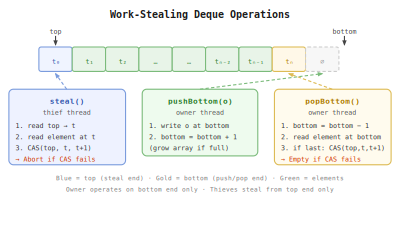
\includegraphics[width=\linewidth]{deque_ops}
  \caption{The three operations of the work-stealing deque.}
  \label{fig:deque-ops}
\end{figure}

\begin{itemize}[noitemsep, nosep]
    \item pushBottom o: which pushes o to the bottom end of the deque
    \item popBottom: pops an object from the bottom of the deque; if the
        deque is empty, an Empty value is returned.
    \item steal: if a stealing process attempts to deque a value from the local
        deque, one of the three values can be returned:
       \begin{itemize}[noitemsep]
           \item if a task is successfully stolen from the top end of the deque,
                 then that task is returned
           \item if the local deque is empty, then an Empty value is returned
           \item if the stealing process loses out to another stealing process,
                 then an Abort value is returned.
      \end{itemize}
\end{itemize}

The salient feature of the ABP algorithm is that the arrays backing the deques
are of fixed size. Changing these arrays to be cyclic - where the top and
the bottom indices are reset to point to the beginning of the array when the
deque becomes empty - makes overflow less frequent but does not rule out its
occurrence. A subsequent design from \cite{hendler2005dynamic} used a list of
arrays to address this problem but these arrays were not cyclic and using the
list of arrays presented a more complicated algorithm to reason about in
terms of time and space complexity.

The Chase-Lev algorithm addresses the overflow problem by using dynamic cyclic
arrays. The only practical restriction on deque size is integer overflow in the
address space.  In our OCaml implementation, integers have a runtime
representation of 63 bits, giving a maximum value of
$2^{63} - 1 \approx 9.22 \times 10^{18}$.

Given the operation rate quoted in the paper of $4 \times 10^{9}$ operations per second,
the time until deque index overflow occurs is:

\[
\frac{2^{63} - 1}{4 \times 10^{9}} \approx 2.30 \times 10^{9} \text{ seconds}
\]

Converting to years, using $365.25 \times 24 \times 3600 \approx 3.156 \times 10^{7}$
seconds per year:

\[
\frac{2.30 \times 10^{9}}{3.156 \times 10^{7}} \approx 73 \text{ years}
\]

In practical terms, integer overflow is not a concern for this algorithm on
modern systems.

In our implementation, deques are implemented using cyclic array whose ends are indicated by two
indices where:
\begin{itemize}[noitemsep, nosep]
    \item top: is the first element at the top end of the deque. This end has
    first-in-first-out (FIFO) behaviour and is incremented on every steal
    operation.
\item bottom: is the \emph{next available} slot in the array where a new element
    will be pushed. This index is incremented on every \texttt{pushBottom} operation.
    This end of the deque had last-in-first-out (LIFO) behaviour and so operates
    like a stack.
\end{itemize}

The deque is empty when the \texttt{bottom} is less than or equal to \texttt{top}.

The deque size increases when items are pushed into it. If the current array is
full, a new array with a specified larger size is created. The elements from the
current array are copied over into this new, bigger array. Lastly, the new item
is pushed into this expanded array. The inverse occurs when items are popped
from the deque. If the number of elements in the deque is determined to be less
than a heuristic based on the deque size relative to a predetermined constant,
then the circular array is shrunk to a lesser size. Again, array elements are
copied over to this new, smaller array with the popped element no longer in it.

Arrays backing deques are circular i.e. items are stored indexed modulo to the
array size. On growing the array, moving items into the newer, larger-sized
array, there is no need to update top or bottom although one must always keep in
mind that the actual array indices in this array may be different.

The top and bottom indices operate on opposite ends of the deque and only
contend when the last element can be popped by the local process or stolen
by another process. For this, top is only ever modified by the \texttt{steal}
operation and its value is never decremented indicating a linearized timeline of
items stolen from one end of the deque. With the \texttt{top} index never decremented,
no separate tag field is needed to be stored in the deque to solve the ABA
problem that occured in earlier work-stealing algorithms.

% =============================================================================
\section{Tasks Undertaken}
\label{sec:tasks}
% =============================================================================

\subsection{Implementation}
\subsubsection{Deque and Circular Array implementation}

The implementation began with translating the code for deque operations
presented in the \cite{chase2005dynamic} paper from Java to OCaml
(\href{https://github.com/alinab/fork-cs6868_s26/commit/b7bdeac9167f5fbeaee63e81deceaf0c43733d98}{b7bdeac}).

The deque stores all items in the active array data structure which is defined
as an atomic reference as are the top and bottom indices. This is to ensure the
absence of data races between local and stealing processes acting on the deque.

The \texttt{Atomic.compare\_and\_set} is used to ensure that only one among
possibly multiple competing stealing processes can take an item off the top
end of the deque. The process which succeeds returns with the item wrapped in a
Value, others return an Abort indicating an aborted attempt to steal.

In \texttt{steal}, a thief increments \texttt{top} via a successful CAS,
while the owner may concurrently decrement \texttt{bottom} in
\texttt{pop\_bottom}. The deque is empty when \texttt{top} $\geq$
\texttt{bottom}, and the only genuine race occurs when exactly one element
remains — both operations attempt to claim it simultaneously, resolved by
whichever CAS succeeds first.

Based on the code snippets in the \cite{chase2005dynamic} paper, the circular
array only stores the log of the size, not the size itself. This makes the growing
(\href{https://github.com/alinab/fork-cs6868_s26/commit/8324758fc3e51c064bcb5e6a216e97d5cc356c15}{8324758})
and shrinking
(\href{https://github.com/alinab/fork-cs6868_s26/commit/a9f0687fc8eb0b61dc2f059683f209be6a223649}{a9f0687})
of the circular array elegant and only requires copying items from the older to
the expanded or the shrunk array.

The \texttt{Deque.perhaps\_shrink} method shrinks the
array if the number of elements in the deque is less than 1/K of the array size,
where K >= 3. This ensures that when the array is shrunk and halved in size, the
number of elements are less than 1/3rd of the array. This ensures that there's
enough free space for newer items to be pushed to the deque and no need to
expand the array soon after shrinking.


\subsubsection{Scheduler implementation}

The scheduler (\href{https://github.com/alinab/fork-cs6868_s26/blame/work-steal/work-steal/lib/scheduler.ml}{0b98700})
whose constituent types are shown above is a parallel work-stealing
one where each domain (worker) owns a local double-ended deque of tasks. Worker domains
push and pop tasks from the bottom of their own deque in a lock-free manner,
while idle workers choose another domain's deque to steal tasks from using a
compare-and-swap (CAS) instruction.

This design ensures that synchronization cost is proportional to stealing
frequency rather than task frequency, since the local push and pop requires no
cross-domain coordination.

Each task receives a context (\texttt{ctx}) carrying a reference to the
shared pool, which holds the array of per-worker deques, a count of pending
tasks yet to complete, and a count of successful steals. Tasks are decomposed
via \texttt{fork}, which wraps a computation in a new task, pushes it onto
the owner's local deque, increments the pending count, and immediately returns
a \texttt{future} — a placeholder that will be filled with the result when the
task eventually executes.  \texttt{join} blocks logically on the spawned task
but keeps the domain productive by continuing to execute or steal tasks until
the awaited future is filled. It runs the same work-stealing loop — popping
from the local deque or stealing from a victim — until the awaited future is ready.
This ensures that synchronisation cost is proportional to stealing
frequency rather than task frequency: local \texttt{push\_bottom} and
\texttt{pop\_bottom} require no cross-domain coordination, and the
CAS is only invoked during a steal or when the last element of a deque is contested.

\subsection{Testing and verification}

\subsubsection{QCheck-Lin testing}

The QCheck-Lin test involved developing a model using the
\texttt{Lin\_domain.Make\_internal} functor and
\href{https://github.com/alinab/fork-cs6868_s26/blame/work-steal/work-steal/test/test_deque_qcheck_lin.ml}{
types} for deque commands and results.

The initial model was incorrect as all deque operations were spread across
two parallel domains, violating the deque's owner/thief constraint where only
one domain can call \texttt{push\_bottom} and \texttt{pop\_bottom}
while \texttt{steal} is called by the other domain in parallel. Also,
returning a \texttt{Deque.Abort} value has no sequential equivalent causing
spurious linearizability failures i.e. only if an
actual Value is returned can a \texttt{pop\_bottom} or an \texttt{steal}
operation be successful. An empty deque or a failed steal attempt never
actually return a value and must be treated as semantically equal results
when concurrent operations on parallel domains are executed.

Running the test on a TSAN-enhanced opam switch did help trace and pinpoint
an error (fixed in
\href{https://github.com/alinab/fork-cs6868_s26/commit/5d917e0d987c3c1a6a507697c65432e02636c1ce}{5d917e0}).
TSAN was throwing up a data race on the \texttt{push\_bottom} operation. The problem
was that \texttt{push\_bottom} was reading the \texttt{active\_array}
i.e. the array backing the deque and potentially growing it. However, a
concurrent steal operation reading the \texttt{active\_array} between the
\texttt{grow} operation and the \texttt{put\_item} operation would have seen
the older, stale array and read an element from it while the owner
was writing to the new one. The fix was to ensure the array swap was published
atomically via \texttt{Atomic.set} before any writes to the new array, so that any
concurrent \texttt{steal} either sees the old array in its entirety or the
new one — never an intermediate state.

\subsubsection{QCheck-STM testing}

The QCheck-STM test required a more careful design than the Lin test because
STM checks exact values against a sequential model rather than just
linearizability. The sequential model represents the deque as a plain int list
where the front is the steal end (top index) and the back is the push/pop end
(bottom index). \texttt{next\_state} advances the model by appending to the
back for the \texttt{push\_bottom} operation, removing from the back for the
\texttt{pop\_bottom} operation, and removing from the front for the
\texttt{steal} operation.

A major hurdle was navigating STM's GADT-based \texttt{res} type — the Res
constructor wraps values alongside a \texttt{ty\_show} combinator, and naive pattern
matching inside the \texttt{postcond} caused OCaml's type checker to report ambiguous
type escaping errors. The fix was to compute expected values as plain int option
values outside the GADT match before comparing.

The second hurdle was the same owner/thief constraint from the Lin test -
\texttt{STM\_domain.Make} distributes all operations across both parallel domains,
causing \texttt{push\_bottom} and \texttt{pop\_bottom} to race concurrently
and crash with index out of bounds. The fix was to use the \texttt{arb\_triple}
with separate generators for each domain similar to the qcheck-lin test.

% =============================================================================
\section{Evaluation}
\label{sec:evaluation}
% =============================================================================

\subsection{Experimental Setup}

All benchmarks were run on a personal machine running macOS with an
Apple M-series processor. The machine has four performance cores and four
efficiency cores with a shared L2 cache. All measurements were taken using
\texttt{OCaml 5.4} compiled to native code with optimisation flag \texttt{-O3}.

Each benchmark configuration was run $10$ times after $3$ warm-up runs whose
results were discarded.  To handle noise, we report the mean wall-clock time $\bar{t}$, the standard
deviation $\sigma$, and the minimum observed time $t_{\min}$ across the 10
measured runs. Wall-clock time is measured using \texttt{Unix.gettimeofday}
which has microsecond resolution on the test machine. Each run uses a freshly
generated random array as input to avoid cache effects from reusing the same
data across runs.

%Speedup is computed relative to a warmed sequential baseline using
%\texttt{Array.sort} with the standard \texttt{compare} function:
%
%\[
%  \text{speedup} = \frac{\bar{t}_{\text{sequential}}}{\bar{t}_{\text{parallel}}}
%\]
%
All benchmarks are run for both the work-stealing scheduler and the
mutex-protected shared-queue scheduler described in
\cref{sec:tasks}, under varying worker counts (1, 2, 4, 8, 16) and
task granularity thresholds

%%===========================================================================
\subsection{Fibonacci benchmarks}
\begin{figure}[h]
   \centering
   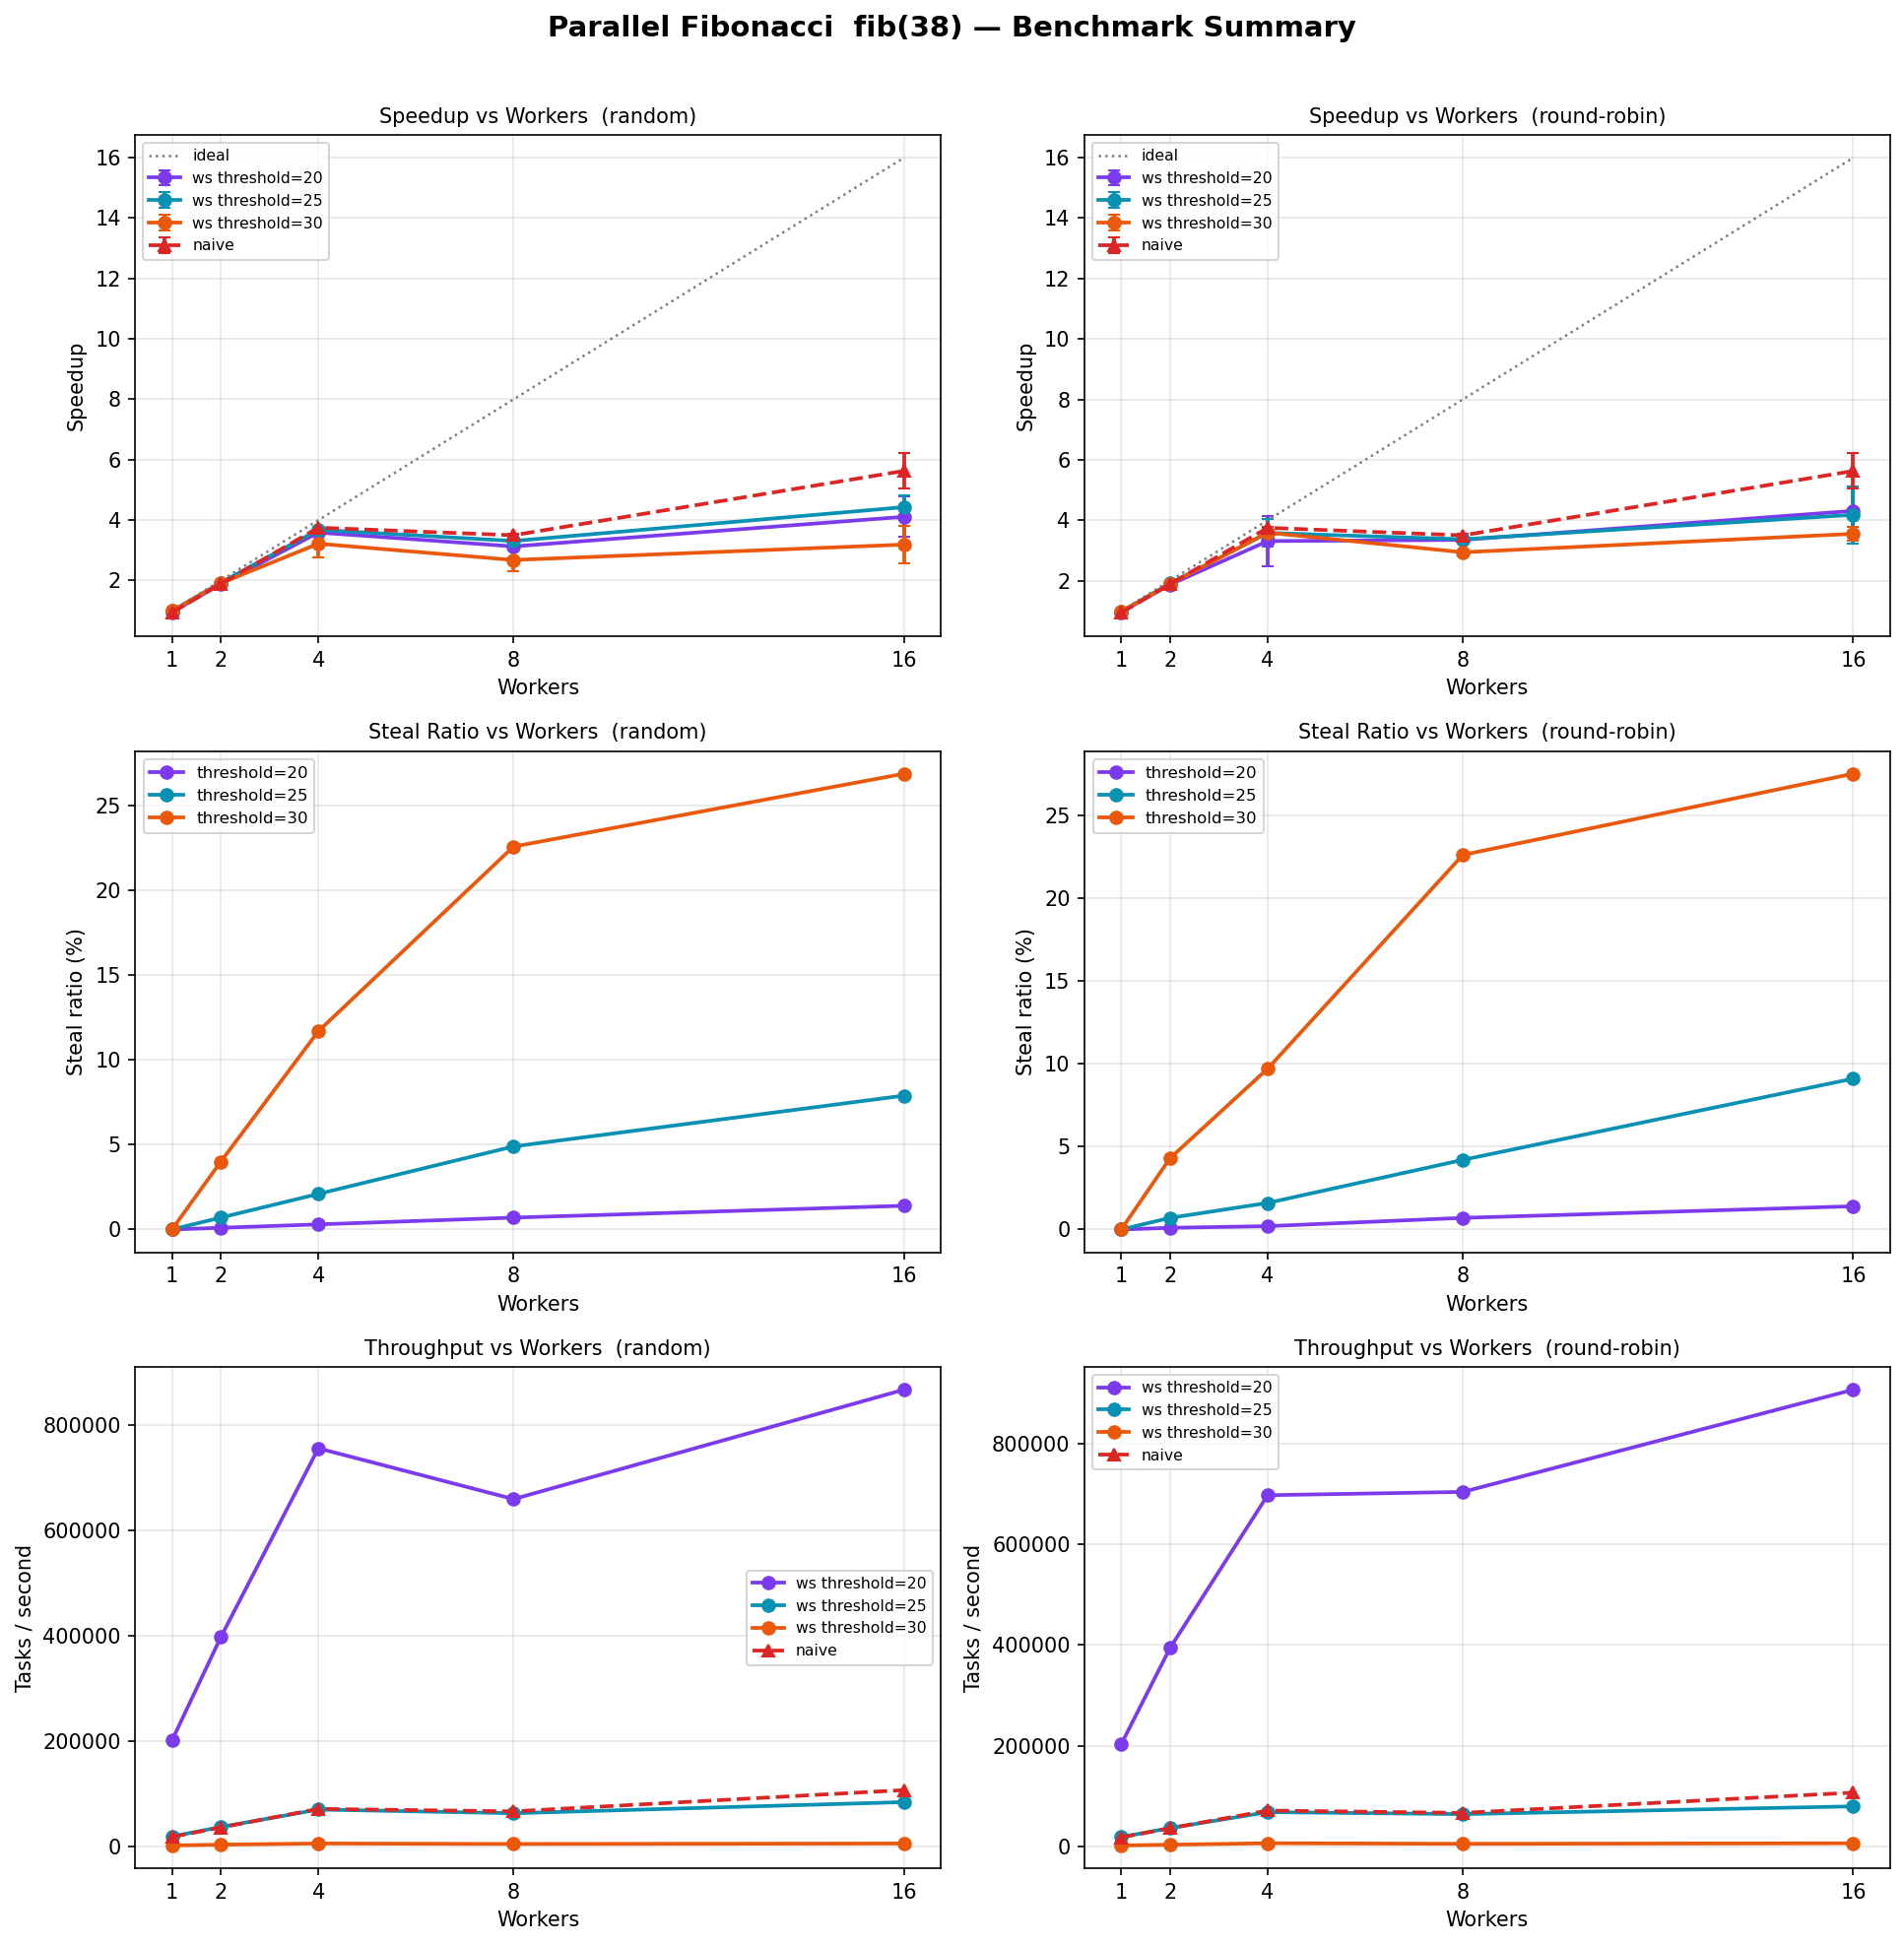
\includegraphics[width=0.9\linewidth]{outputs/fib_combined_throughput.png}
   \caption{Fibonacci benchmarks}
   \cref{fig:fibonacci}
   \label{fig:fibonacci}
 \end{figure}

For the Fibonacci problem, the benchmarks do not show any significant
differences in speedups between the two policies, random vs round-robin. The
benchmarks do show higher steal ratios given more workers as more workers means
each worker gets fewer local tasks on average — the probability of going idle
and needing to steal increases with each additional worker. This confirms that
for a
balanced compute-bound workload the choice of victim selection strategy has
little effect on overall performance.

With threshold=20 there are 67,645 tasks spread across 16 workers —
each worker gets roughly 4,000 tasks locally and rarely needs to steal.
With threshold=30 there are only 545 tasks — 16 workers competing for 545 tasks
means many workers finish their local tasks quickly and must steal from others.

Task throughput is marginally higher under round-robin than random victim
selection, likely because round-robin eliminates redundant steal attempts
on already-empty deques by always targeting the next worker in sequence.

%%===========================================================================
\subsection{Mergesort benchmarks}
\begin{figure}[h]
   \centering
   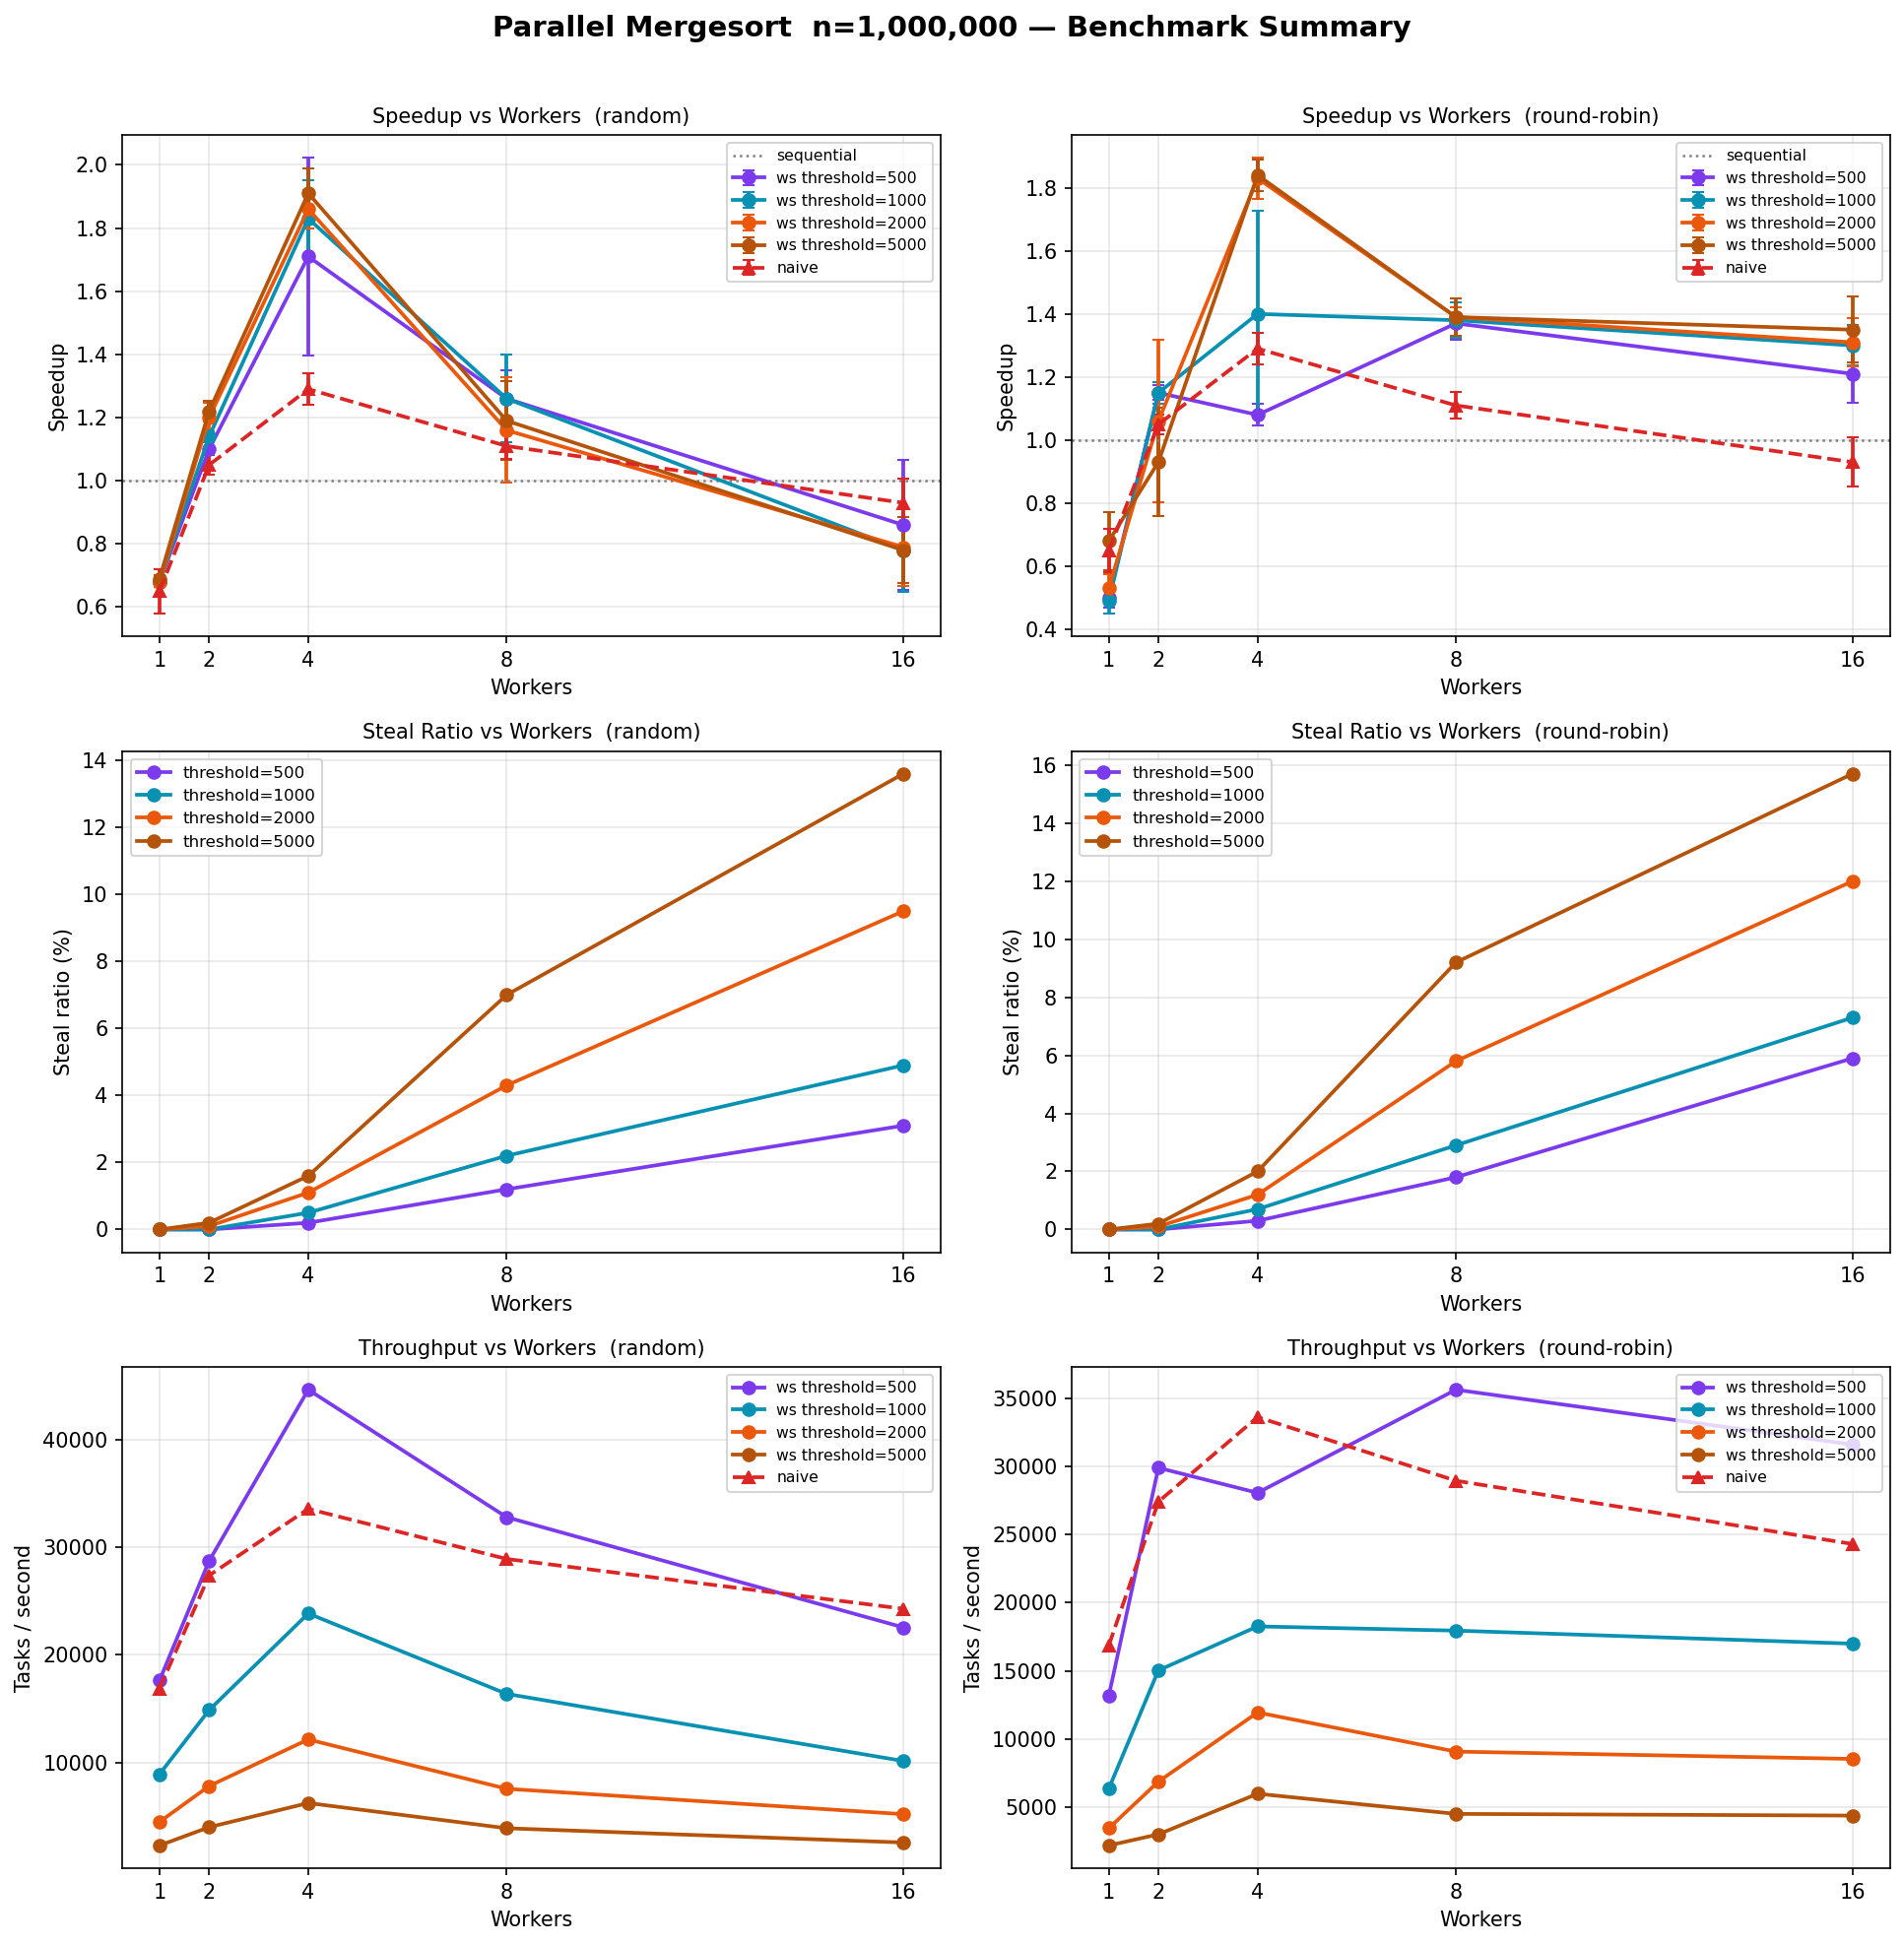
\includegraphics[width=0.9\linewidth]{outputs/mergesort_combined_throughput.png}
   \caption{Mergesort benchmarks}
   \cref{fig:mergesort}
   \label{fig:mergesort}
 \end{figure}

The mergesort benchmarks show that beyond 4 domains, memory contention increases
and throughput degrades i.e. adding more workers hurts rather than it helps execution.
In the naive scheduler, the mutex protecting the shared queue becomes a severe
bottleneck when combined with memory bus contention. Work-stealing avoids this
by keeping operations local to the deques.

The round-robin panel shows a large error bar at workers=4 with threshold=5000
— this reflects a risk of deadlock (livelock) where workers cycle through each
other without finding work when tasks are scarce.

Mergesort's unbalanced merge steps mean coarser tasks have very different
execution times — a top-level merge of 500k elements takes far longer than a
leaf merge of 500 elements. This imbalance drives more stealing at higher thresholds.

The point where naive throughput crosses below work-stealing is at workers=8 for
random and workers=4 for round-robin — this is the practical threshold above
which work-stealing is worth the additional complexity for this workload.

%%===========================================================================
\subsection{Parallel map benchmarks}
\begin{figure}[h]
   \centering
   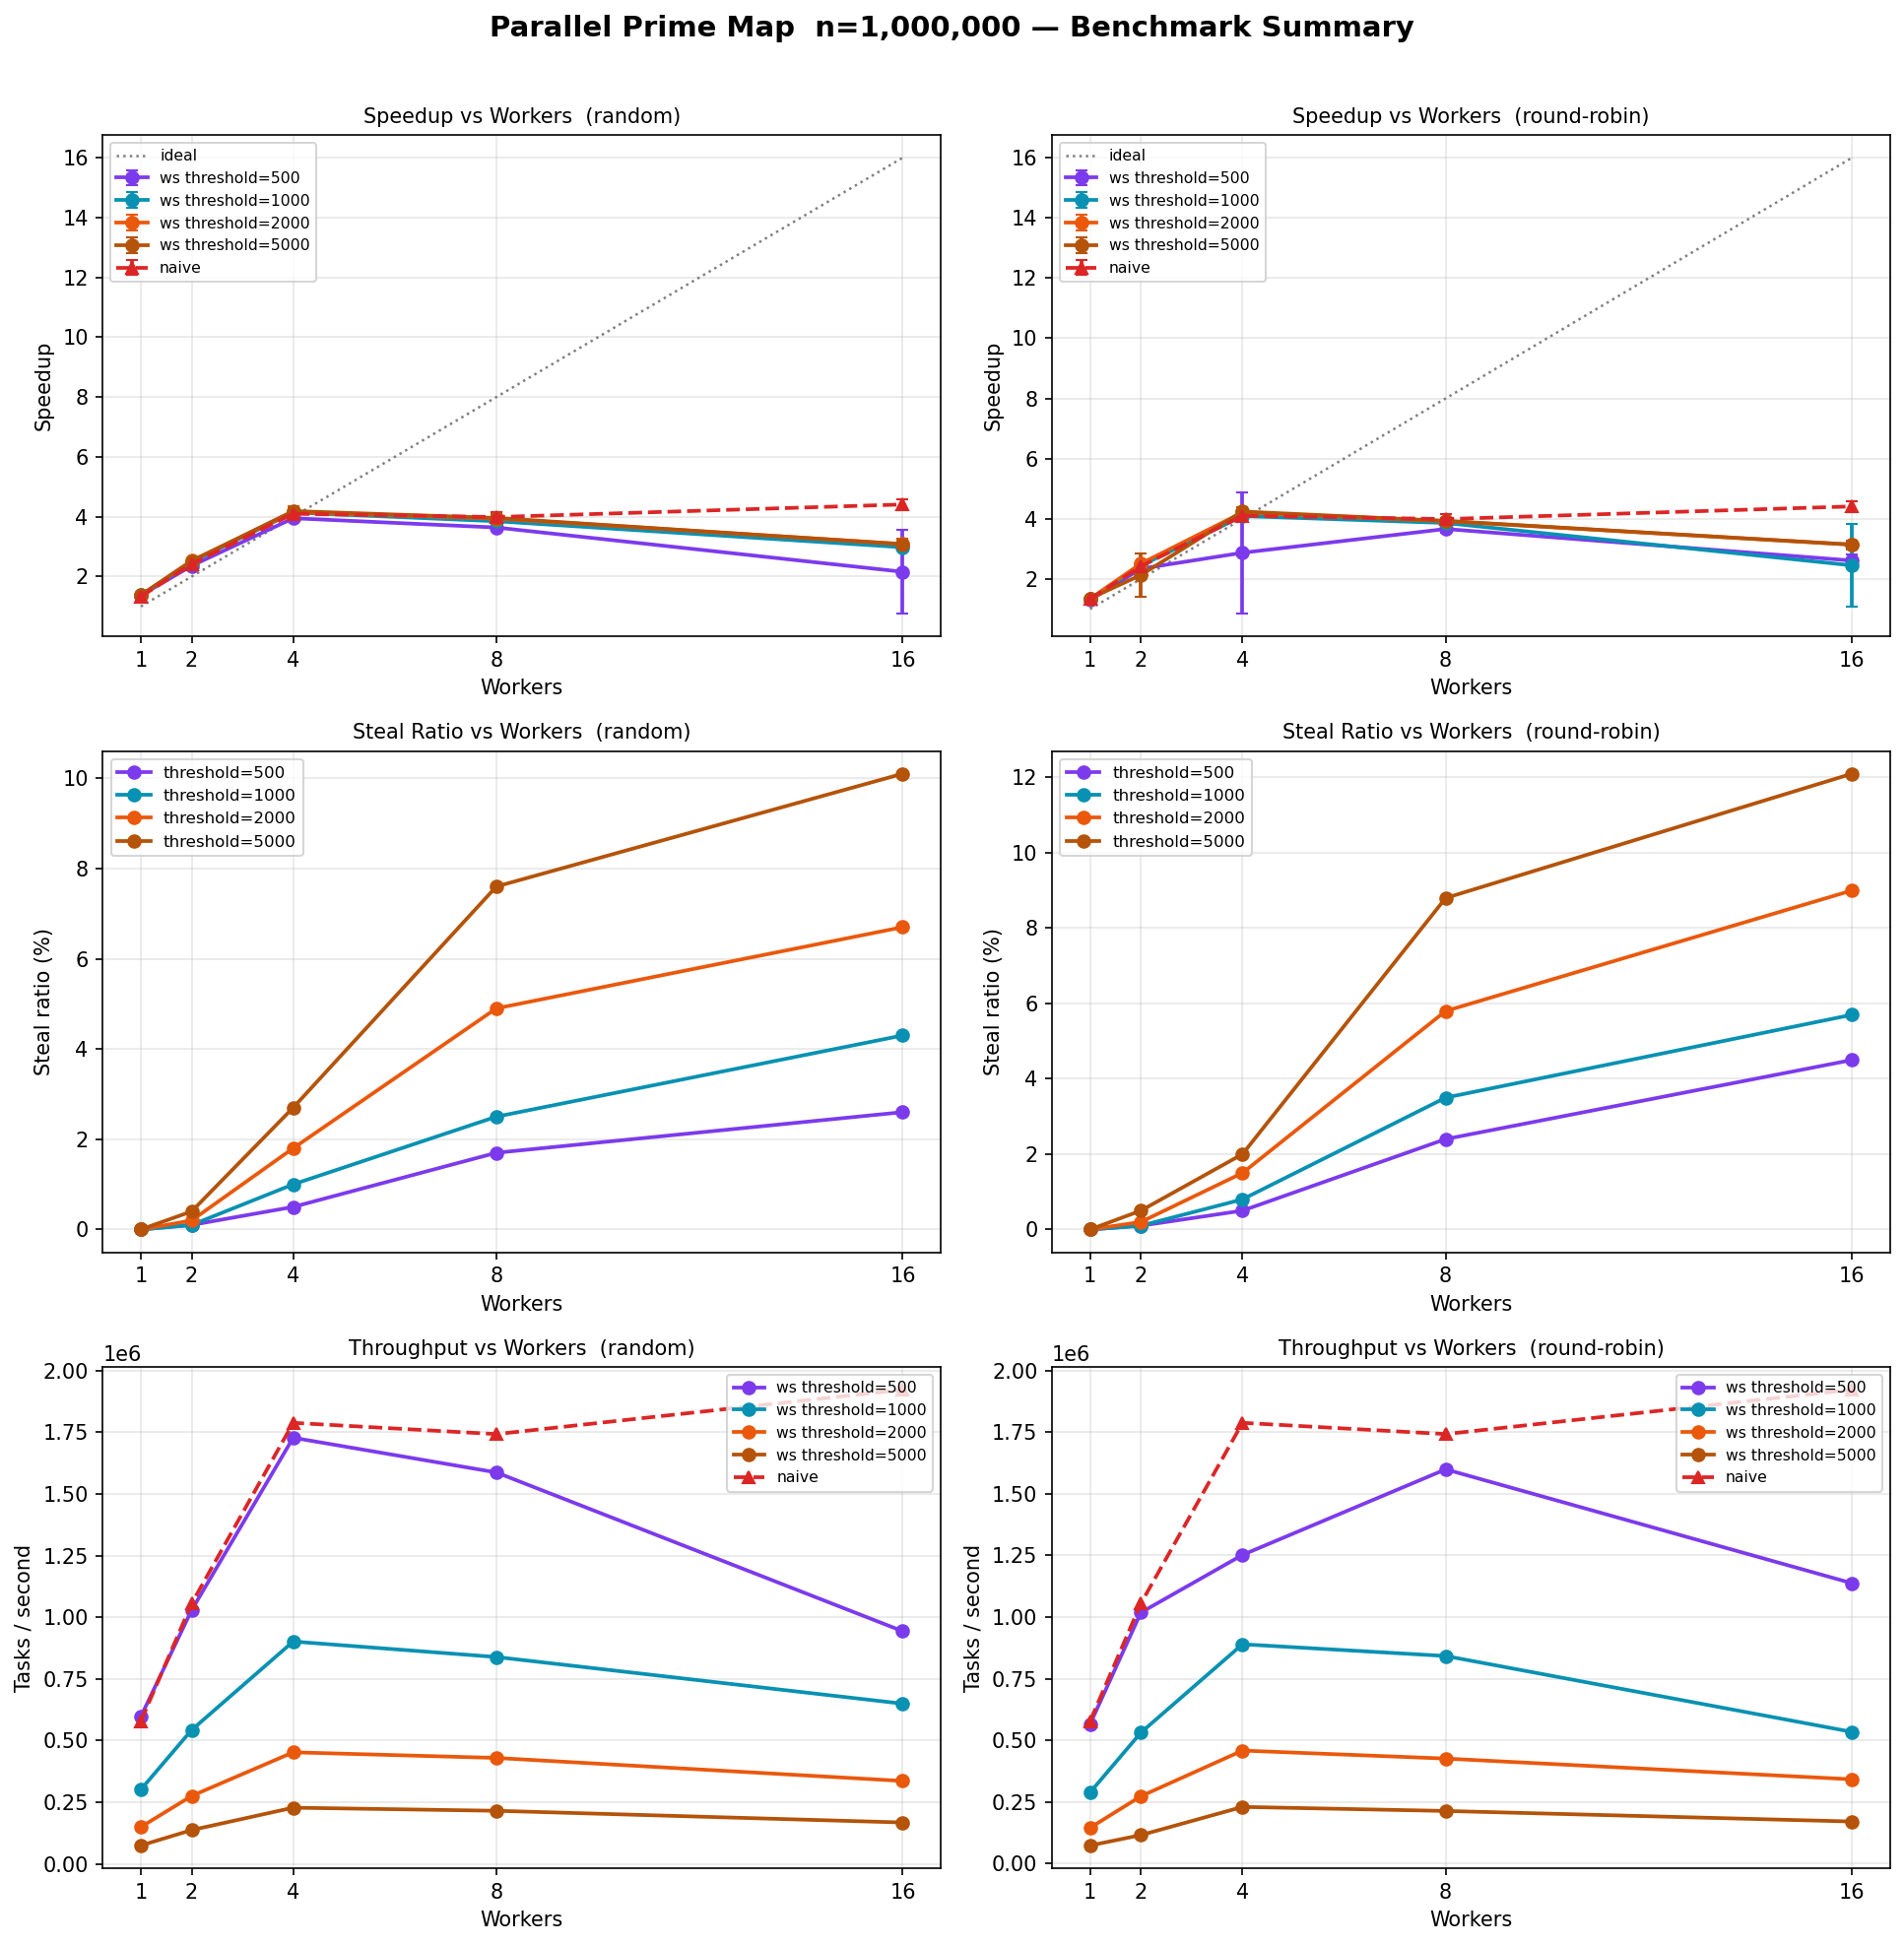
\includegraphics[width=0.9\linewidth]{outputs/map_combined_throughput.png}
   \caption{Parallel map benchmarks}
   \cref{fig:parmap}
   \label{fig:parmap}
 \end{figure}

The naive outperforms work-stealing at all worker counts beyond 4.
The primality test is more balanced than mergesort — each array chunk does
roughly similar work — so the naive queue distributes work well without
needing rebalancing.

The large error bar at workers=4, threshold=500 in the round-robin panel reflects
the same deadlock instability seen in mergesort — with only ~ 20000 tasks and
4 workers cycling in sequence, some runs hit contention while others do not.

The map throughput is orders of magnitude higher than mergesort because each
task is much smaller — checking primality of one chunk takes microseconds vs
milliseconds for sorting. This makes the throughput difference between thresholds
very dramatic.

Naive throughput is remarkably stable across worker counts — the balanced workload
means the mutex is rarely contested and workers always find tasks immediately.
The throughput drop at 16 workers reflects increased steal overhead — with 16
workers competing for a balanced workload, more time is spent in
\texttt{try\_steal} failing to find work than actually executing tasks.

The prime map sits between fibonacci and mergesort — compute-bound like fibonacci
but balanced like a simple array operation. This balance is why naive performs
well — the paper's work-stealing advantage is most visible for irregular
unbalanced workloads.


% =============================================================================

\section{Reflection on the Use of LLMs}
\label{sec:llm}
% =============================================================================

\paragraph{Tools and models used.}
Claude's Sonnet 4.6 (Adaptive) model was the only one used for the following:
     (1)~translating the deque and circular array code from Java to OCaml
     (2)~working out the design of scheduler especially contexts and pools and
     subsequent implementation; also debugging errors when benchmark programs were run.
     (3)~working out and implementing the qcheck-lin and qcheck-stm tests,
     especially informing us of the $arb\_triple$ function to test parallel deques
     (3)~writing the code for the benchmark programs
     (4)~writing the Python scripts for generating all the output plots

\paragraph{What worked well.}
In terms of helping work out functions, module designs etc., Claude acted
as a teacher in prompting us to think a bit first on what was needed, try to
write the necessary code and help come up with a correction or completely new
piece if one was stuck. In terms of the qcheck test, it was crucial in helping
figure out the design for testing deques in parallel with limitations on their
actions (i.e. a deque can never steal from itself). Claude did away the major
tedium and time it would have taken to painstakingly write benchmark programs
and plot the outputs.


\paragraph{What did not work.}
Minor things such as suggesting OCaml's \texttt{Atomic.fetch\_and\_add} when
\texttt{Atomic.incr} or \texttt{Atomic.decr} is perfectly fine.
The non-adaptive model for Sonnet made a mistake when asked to generate an example
from the paper - it thought \texttt{pop\_bottom} to occur from the top index
of the deque, an impossibility.

\paragraph{What was surprising.}
The patience with which it would help think through something. This is our first
major project where an LLM has been used to think through and work out a
research paper, so that was helpful and pleasant. Claude was
surprisingly very good at helping work out the scheduler design and
implementation but needing help simplifying basic functions was unexpected.

\paragraph{What was difficult.}
While Claude helped in the translation of paper's code for deques from Java to
OCaml, the order for writing to/reading from arrays, correctly updating their
indices had to be carefully reasoned about. While testing one or two errors
cropped up in these functions and having worked through the code step-by-step
helped debug it.

\paragraph{Your overall assessment.}
While Claude was crucial in helping work through major parts of and design the
project in a short time, it would be in our long-term benefit to approach the
problem more slowly, look at existing codebases, struggle a bit more, only then
approach a tool such as Claude because it can be very dangerous to use it as an
easy resource to come up with answers without really grappling with the problem
in the first place.

% =============================================================================
\section{Conclusions}
\label{sec:conclusions}
% =============================================================================

Work-stealing's advantage is most pronounced for memory-bound
unbalanced workloads such as parallel mergesort, where dynamic rebalancing
avoids the mutex contention that cripples the naive scheduler at high worker
counts. For compute-bound, balanced workloads such as Fibonacci and prime map,
the naive scheduler is surprisingly competitive — and superior at very high
worker counts — because workers rarely go idle and the mutex is rarely contested.

The steal ratio data validates the algorithm's theoretical foundation: across
all benchmarks and configurations, between 0\% and 27\% of tasks were stolen,
meaning at least 73\% executed locally without any cross-domain synchronisation.
\texttt{push\_bottom} and \texttt{pop\_bottom} are lock-free on the owner's
local deque; the expensive CAS is only invoked during a steal or when the last
element is contested.

Random victim selection is more stable than round-robin across all benchmarks.
At high worker counts round-robin's deterministic cycling causes contention when
multiple workers target the same victim, leading to higher variance and
occasional livelock under coarse task granularity.

Task granularity has a consistent effect on performance: fine-grained tasks
increase parallelism and throughput but add scheduler overhead per unit of
computation. The crossover threshold below which sequential outperforms parallel
is approximately \texttt{threshold=1000} for mergesort and
\texttt{threshold=20} for Fibonacci, confirming that minimum viable task size
depends heavily on computational intensity.

Given more time, profiling tools for cache and memory analysis would help
pinpoint threshold tipping points, and additional benchmarks would broaden the
evaluation. As a natural extension, implementing a shared buffer pool — and
comparing it against an equivalent Rust implementation using
\href{https://docs.rs/crossbeam-deque/latest/crossbeam_deque/}{\texttt{crossbeam}}
or a from-scratch implementation — would help us understand acquire-release semantics
much better as well as the and the practical differences between
garbage-collected and manually managed memory models.

% =============================================================================
\section*{Contributions}
\label{sec:contributions}
% =============================================================================

% Required. Percentages must sum to 100. Every member should contribute.

\begin{center}
\begin{tabular}{@{}lcl@{}}
\toprule
\textbf{Member} & \textbf{Contribution (\%)} & \textbf{Main responsibilities} \\
\midrule
Alina Banerjee  & \% & \\
Member Two      & \% & \\
Member Three    & \% & \\
\midrule
\textbf{Total} & \textbf{100\%} & \\
\bottomrule
\end{tabular}
\end{center}

% =============================================================================
\bibliographystyle{plainurl}
\bibliography{references}
% =============================================================================

\end{document}
